% Chapter 6: Application Studies

\chapter{Application Studies}
\label{ch:sixth} % For referencing the chapter elsewhere, use \autoref{ch:name}
\label{chapter:codeGeneration-evaluation}
\addtocontents{lof}{\protect\vspace{\beforebibskip}}%
\addtocontents{lol}{\protect\vspace{\beforebibskip}}%

\lettrine[lines=3, loversize=0.1]{I}{n this chapter} we present application studies evaluating the performance of the \OpenCL code generated from pattern-based expressions using our systematic code generation approach presented in the previous chapter.
We first discuss our experimental setup used for the runtime experiments.
We will then start our evaluation by looking at the parallel reduction example which we used throughout the previous chapter and compare the performance of the manually optimized \OpenCL implementations against the systematically generated code.
We will discuss a brief case study showing how the rewrite rules can be applied automatically and how effective such an automatic search strategy is for a simple application example.
We will then investigate application examples from linear algebra, physics, and mathematical finance.

For all applications we show performance results comparing the generated \OpenCL code against vendor provided libraries and manually tuned \OpenCL code.

\section{Experimental Setup}
We used three hardware platforms: an Nvidia GeForce GTX 480 \GPU, an AMD Radeon HD 7970 \GPU, and a dual socket Intel Xeon E5530 server with 8 cores in total.
We used the latest \OpenCL runtime from Nvidia (\CUDA-SDK 5.5), AMD (AMD-APP 2.8.1) and Intel (XE 2013 R3).
The \GPU drivers installed were 310.44 for Nvidia and 13.1 for AMD on our Linux system.

We use the profiling \APIs from \OpenCL and \CUDA to measure kernel execution time and the \textit{gettimeofday} function for the \CPU implementation.
We exclude the data transfer time to and from the \GPU in all runtime numbers reported in this chapter, as we want to focus on the quality of the generated \OpenCL kernel code.
We repeat each experiment 100 times and report median runtimes.




\section{Parallel Reduction}
In this section we evaluate the performance of three of the low-level expressions presented in \autoref{sec:deriving:reduce} performing a parallel summation of an array.
These expressions resemble corresponding \OpenCL code provided by Nvidia discussed at the beginning of \autoref{chapter:codeGeneration}.
All three expressions have been systematically derived from the high-level expression for the parallel summation:
\begin{equation*}
  vecSum = \reduce\ (+)\ 0
\end{equation*}
The formal derivations are shown in \autoref{chapter:derivations}.

\begin{figure*}[t]
\captionsetup[subfigure]{justification=justified,singlelinecheck=false}

\begin{subfigure}[b]{\linewidth}
\vspace{.4em}
\begin{minipage}{.05\linewidth}
\caption{}
\label{fig:reduce:expr:1}
\end{minipage}
\hfill
\begin{minipage}{.9\linewidth}
\begin{lstlisting}[mathescape, basicstyle=\small\rmfamily]
$vecSum = \reduce \circ \join \circ \mapWorkgroup\ \big($
    $\join \circ \toGlobal\ (\mapLocal\ (\mapSeq\ \id)) \circ \splitN\ 1\ \circ$
    $\iterateN\ 7\ (\join \circ \mapLocal\ (\reduceSeq\ (+)\ 0) \circ \splitN\ 2)\ \circ$
    $\join \circ \toLocal\ (\mapLocal\ (\mapSeq\ \id)) \circ \splitN\ 1$
  $\big) \circ \splitN\ 128$
\end{lstlisting}
\end{minipage}
\end{subfigure}

\begin{subfigure}[b]{\linewidth}
\vspace{0em}
\begin{minipage}{.05\linewidth}
\caption{}
\label{fig:reduce:expr:2}
\end{minipage}
\hfill
\begin{minipage}{.9\linewidth}
\begin{lstlisting}[mathescape, basicstyle=\small\rmfamily]
$vecSum = \reduce \circ \join \circ \mapWorkgroup\ \big($
    $\join \circ \toGlobal\ (\mapLocal\ (\mapSeq\ \id)) \circ \splitN\ 1\ \circ$
    $\iterateN\ 7\ \big(\ \lambda\ xs\ .\ \join \circ \mapLocal\ (\reduceSeq\ (+)\ 0) \circ \splitN\ 2\ \circ$
                $\reorderStride\ ((size\ xs)/2)\ \$\ xs\ \big)\ \circ$
    $\join \circ \toLocal\ (\mapLocal\ (\reduceSeq\ (+)\ 0)) \circ \splitN\ 2\ \circ$
    $\reorderStride\ 128$
  $\big) \circ \splitN\ (2\times 128)$
\end{lstlisting}
\end{minipage}
\end{subfigure}

\begin{subfigure}[b]{\linewidth}
\vspace{0em}
\begin{minipage}{.05\linewidth}
\caption{}
\label{fig:reduce:expr:3}
\end{minipage}
\hfill
\begin{minipage}{.9\linewidth}
\begin{lstlisting}[mathescape, basicstyle=\small\rmfamily]
$vecSum = \reduce \circ \join \circ \mapWorkgroup\ \big($
    $\join \circ \toGlobal\ (\mapLocal\ (\mapSeq\ \id)) \circ \splitN\ 1\ \circ$
    $\join \circ \mapWarp\ \big($
      $\join \circ \mapLane\ (\reduceSeq\ (+)\ 0) \circ \splitN\ 2\ \circ \reorderStride\ 1\ \circ$
      $\join \circ \mapLane\ (\reduceSeq\ (+)\ 0) \circ \splitN\ 2\ \circ \reorderStride\ 2\ \circ$
      $\join \circ \mapLane\ (\reduceSeq\ (+)\ 0) \circ \splitN\ 2\ \circ \reorderStride\ 4\ \circ$
      $\join \circ \mapLane\ (\reduceSeq\ (+)\ 0) \circ \splitN\ 2\ \circ \reorderStride\ 8\ \circ$
      $\join \circ \mapLane\ (\reduceSeq\ (+)\ 0) \circ \splitN\ 2\ \circ \reorderStride\ 16\ \circ$
      $\join \circ \mapLane\ (\reduceSeq\ (+)\ 0) \circ \splitN\ 2\ \circ \reorderStride\ 32$
    $\big) \circ \splitN\ 64\ \circ$
    $\join \circ \mapLocal\ (\reduceSeq\ (+)\ 0) \circ \splitN\ 2\ \circ \reorderStride\ 64\ \circ$
    $\join \circ \toLocal\ (\mapLocal\ (\reduceSeq\ (+)\ 0))\ \circ$
    $\splitN\ (blockSize/128)\ \circ \reorderStride\ 128$
  $\big) \circ \splitN\ blockSize$
\end{lstlisting}
\end{minipage}
\end{subfigure}

\caption{Three low-level expressions implementing parallel reduction.}
\label{fig:reduce:expr}
\end{figure*}


\autoref{fig:reduce:expr} shows the three expressions we will use for our performance comparison.
The first expression (\autoref{fig:reduce:expr:1}) corresponds to the first unoptimized Nvidia implementation (\autoref{lst:reduce1}),
the second expression (\autoref{fig:reduce:expr:2}) corresponds to the fourth implementation by Nvidia which has some optimizations applied (\autoref{lst:reduce3}), and
the third expression (\autoref{fig:reduce:expr:3}) corresponds to the fully optimized Nvidia implementation (\autoref{lst:reduce6}).


\begin{figure}
  \centering
  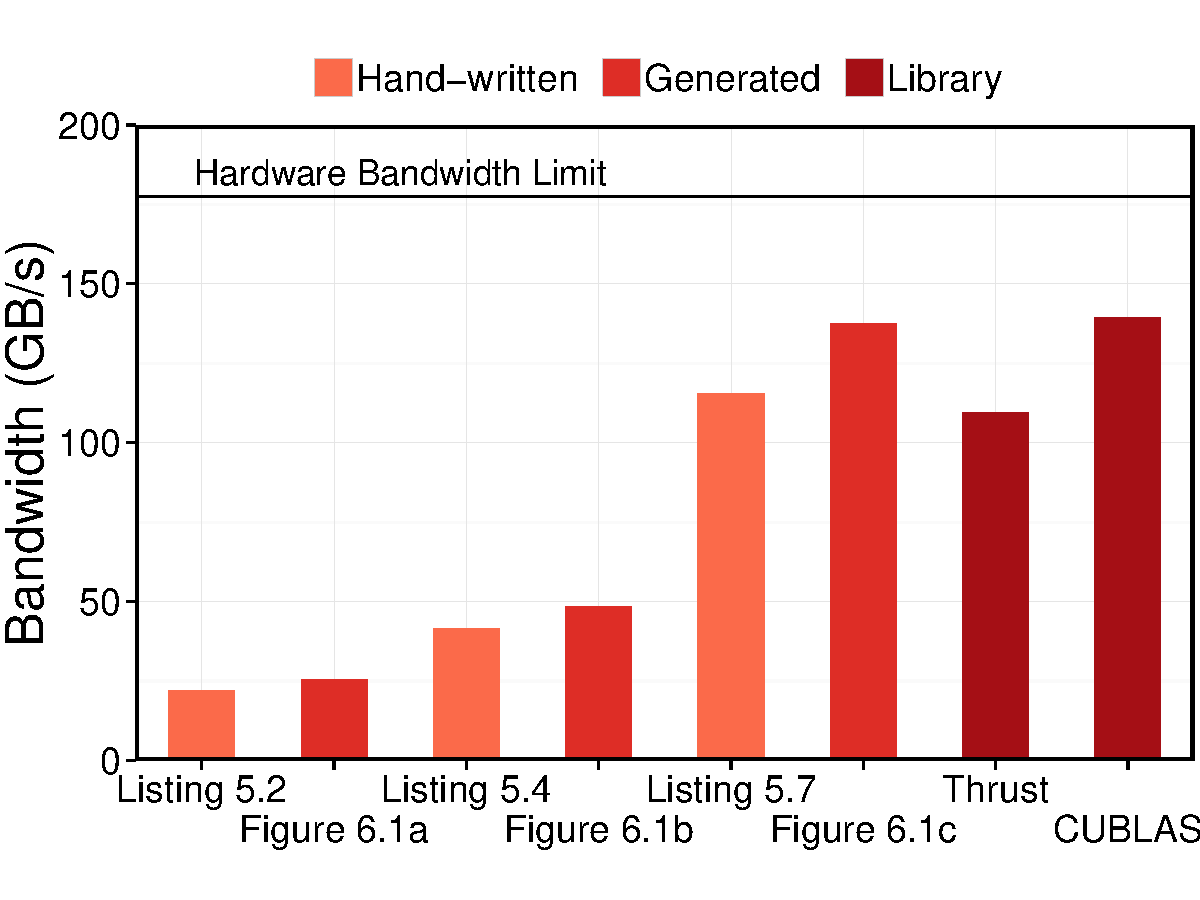
\includegraphics[width=.8\linewidth]{Plots/ReductionGenerator/reduce_runtime.pdf}
  \caption{Performance comparisons for code generated for three low-level expressions against native \OpenCL code.}
  \label{fig:reduce:expr:performance}
\end{figure}

\autoref{fig:reduce:expr:performance} shows the performance of these three versions compared to the corresponding native \OpenCL implementations by Nvidia and two additional libraries providing implementations of parallel reduction on \GPUs.
\CUBLAS~\cite{cuBLAS} represents the \CUDA-specific implementation of \BLAS that only runs on Nvidia hardware.
\BLAS does not implement the parallel reduction but instead we used the \emph{asum} benchmark for our comparison which performs a parallel reduction but in addition applies a function computing the absolute value on every element of the input vector.
We also include a parallel reduction implemented with Thrust~\cite{BellHo2011}, a library for simplified \GPU programming developed by Nvidia and based on \CUDA.

The results are reported in GB/s, \ie, the achieved memory bandwidth which is computed by dividing the input data size in gigabytes by the absolute runtime in seconds.
This metric allows to compare each version against the hardware bandwidth limit, which is marked by a horizontal line at the top of \autoref{fig:reduce:expr:performance}.
The performance of the generated \OpenCL code from our three expressions matches, or even slightly outperforms, the corresponding native \OpenCL implementations written by Nvidia.
These results show that our systematically generated code can offer high performance, once the right set of optimizations -- encoded in our rewrite rules -- is applied.
The performance of our generated code for the fully optimized low-level expression even matches the performance of the highly optimized \CUBLAS library written by Nvidia and outperforms the Thrust library.

\subsection{Automatically Applying the Rewrite Rules}
\label{sec:codeGeneration-evaluation:automatic}

For the parallel reduction benchmark we implemented a prototype search tool which automatically applies the rewrite rules for finding low-level expressions which offer high-performance.
Our prototype tool starts with the high-level expression $\reduce\ (+)\ 0$ and transforms the expression using the rewrite rules and performing runtime experiments with the transformed expressions until a low-level \OpenCL expression is found meeting our performance expectations.
As discussed earlier in \autoref{chapter:codeGeneration} multiple rewrite rules might be valid to be applied to a given expression, therefore, we implemented a simple strategy for deciding which rules to apply.
This simple search strategy is loosely based on Bandit-based optimization~\cite{MesmayRVP09}.

The search is an iterative process.
Given an expression we list all the rewrite rules which are valid to be applied.
We use a Monte Carlo method for evaluating the potential impact of each rule by randomly walking down the search tree.
We execute the code generated from the randomly chosen expressions on the parallel processor using \OpenCL and measure its performance.
The rule that promises the best performance following the Monte Carlo descent is chosen and the expression after the rule has been applied is used as the starting point for the next iteration.
As the rules are chosen randomly the search process is not deterministic and different low-level expressions can be found when applying the search multiple times.

This process is repeated until we reach an expression where there are no rules to be applied to, or a certain depth of the search tree is reached.
In addition to selecting the rules, we also search at the same time for parameters controlling our primitives such as the parameter for the $\splitN\ n$ pattern.
We have limited the choices for these numerical parameters to a reasonable set of appropriate values for our test hardware.

We envision to replace this simplistic search strategy with more advanced techniques in the future.

\paragraph{Found expressions}
We performed the automatic search on all three of our test platforms for the parallel reduction benchmark.

\begin{figure*}[t]
\captionsetup[subfigure]{justification=justified,singlelinecheck=false}

\begin{subfigure}[b]{\linewidth}
\vspace{.4em}
\begin{minipage}{.15\linewidth}
\caption{Nvidia}
\label{fig:reduce:expr:auto:1}
\end{minipage}
\hfill
\begin{minipage}{.8\linewidth}
\begin{lstlisting}[mathescape, basicstyle=\small\rmfamily]
$\reduce \circ \join \circ \join \circ \mapWorkgroup\ \big($
   $\toGlobal\ (\mapLocal\ (\reduceSeq\ (+)\ 0))\circ \reorderStride\ 2048$
  $\big) \circ \splitN\ 128 \circ \splitN\ 2048$
\end{lstlisting}
\end{minipage}
\end{subfigure}

\begin{subfigure}[b]{\linewidth}
\vspace{0em}
\begin{minipage}{.15\linewidth}
\caption{AMD}
\label{fig:reduce:expr:auto:2}
\end{minipage}
\hfill
\begin{minipage}{.8\linewidth}
\begin{lstlisting}[mathescape, basicstyle=\small\rmfamily]
$\reduce \circ \join \circ \asScalar \circ \join \circ \mapWorkgroup\ \big($
    $\mapLocal\ \big(\mapSeq\ (\vect\ 2\ id) \circ$
      $\reduceSeq\ (\vect\ 2\ (+)\ 0)$
    $\big) \circ \reorderStride\ 2048$
  $\big) \circ \splitN\ 128\ \circ \asVector\ 2\ \circ \splitN\ 4096$
\end{lstlisting}
\end{minipage}
\end{subfigure}

\begin{subfigure}[b]{\linewidth}
\vspace{0em}
\begin{minipage}{.15\linewidth}
\caption{Intel}
\label{fig:reduce:expr:auto:3}
\end{minipage}
\hfill
\begin{minipage}{.8\linewidth}
\begin{lstlisting}[mathescape, basicstyle=\small\rmfamily]
$\reduce \circ \join \circ \mapWorkgroup\ \big( \join \circ \asScalar \circ \mapLocal($
    $\mapSeq\ (\vect\ 4\ id) \circ \reduceSeq\ (\vect\ 4\ (+))\ 0$
  $)\circ \asVector\ 4 \circ \splitN\ 32768\big) \circ \splitN\ 32768$
\end{lstlisting}
\end{minipage}
\end{subfigure}

\caption[Low-level expressions performing parallel reduction. These expressions are automatically derived by our prototype search tool from a high-level expression]{Low-level expressions performing parallel reduction. These expressions are automatically derived by our prototype search tool from the  high-level expression $\reduce\ (+)\ 0$.}
\label{fig:reduce:expr:auto}
\end{figure*}

The best performing low-level expression found by applying our automatic search technique are shown in \autoref{fig:reduce:expr:auto}.
The first expression (\autoref{fig:reduce:expr:auto:1}) was found on the Nvidia platform, the second expression (\autoref{fig:reduce:expr:auto:2}) on the AMD platform, and the third expression (\autoref{fig:reduce:expr:auto:3}) on the Intel platform.
We can make several important observations.
The first observation is, that none of the expressions make use of the local memory (although our systems fully support it).
It is common wisdom that using local memory on the \GPU enables high performance and in fact the tuned hand-written implementation by Nvidia uses local memory on the \GPU.
However, as we will see later in the results section, our automatically derived version is able to perform as well without using local memory.
The second key observation is, that each work-item performs a large sequential reduction independent of all other threads, which does not require synchronization and, thus, avoids overheads.

While these observations are the same for all platforms, there are also crucial differences between the different low-level expressions.
Both \GPU expressions make use of the \reorderStride primitive, allowing for coalesced memory accesses.
The AMD and Intel expressions are vectorized with a vector length of two and four respectively.
The Nvidia version does not use vectorization since this platform does not benefit from vectorized code.
On the \CPU, the automatic search picked numbers for partitioning into work-groups and then into work-items in such a way that inside each work-group only a single work-item is active.
This reflects the fact that there is less parallelism available on a \CPU compared to \GPUs.

Interestingly, the results of our search have some redundancies in the expressions.
For example, we perform unnecessary copies on AMD and Intel by performing a \mapSeq with the identity nested inside.
While this does not seem to affect performance much, a better search strategy could probably get rid of these artifacts and might achieve a slightly better performance.


\paragraph{Performance of found expressions}
\autoref{fig:reduce:expr:automatic:performance} shows the performance of the code generated for the three expressions performing a parallel reduction shown in \autoref{fig:reduce:expr:auto}.
The three plots show the performance for the Nvidia platform (on the left), the AMD platform (in the middle), and the Intel platform (on the right).
All plots are scaled according to the hardware bandwidth limit of the platform.
On each platform we compare against a vendor provided, highly tuned implementation of the \BLAS library, where we measured the bandwidth achieved for the \emph{asum} application.
While in the \emph{asum} application an additional operation (applying the absolute value function) is performed for every data item, we showed in \autoref{section:skelcl:evaluation:linearAlgebra} that the performance difference for the parallel reduction benchmark and the \emph{asum} benchmark is negligible when both are implemented properly.
Therefore, we consider the \BLAS implementations as valid contenders for a fair performance comparison.

\begin{figure}
  \centering
  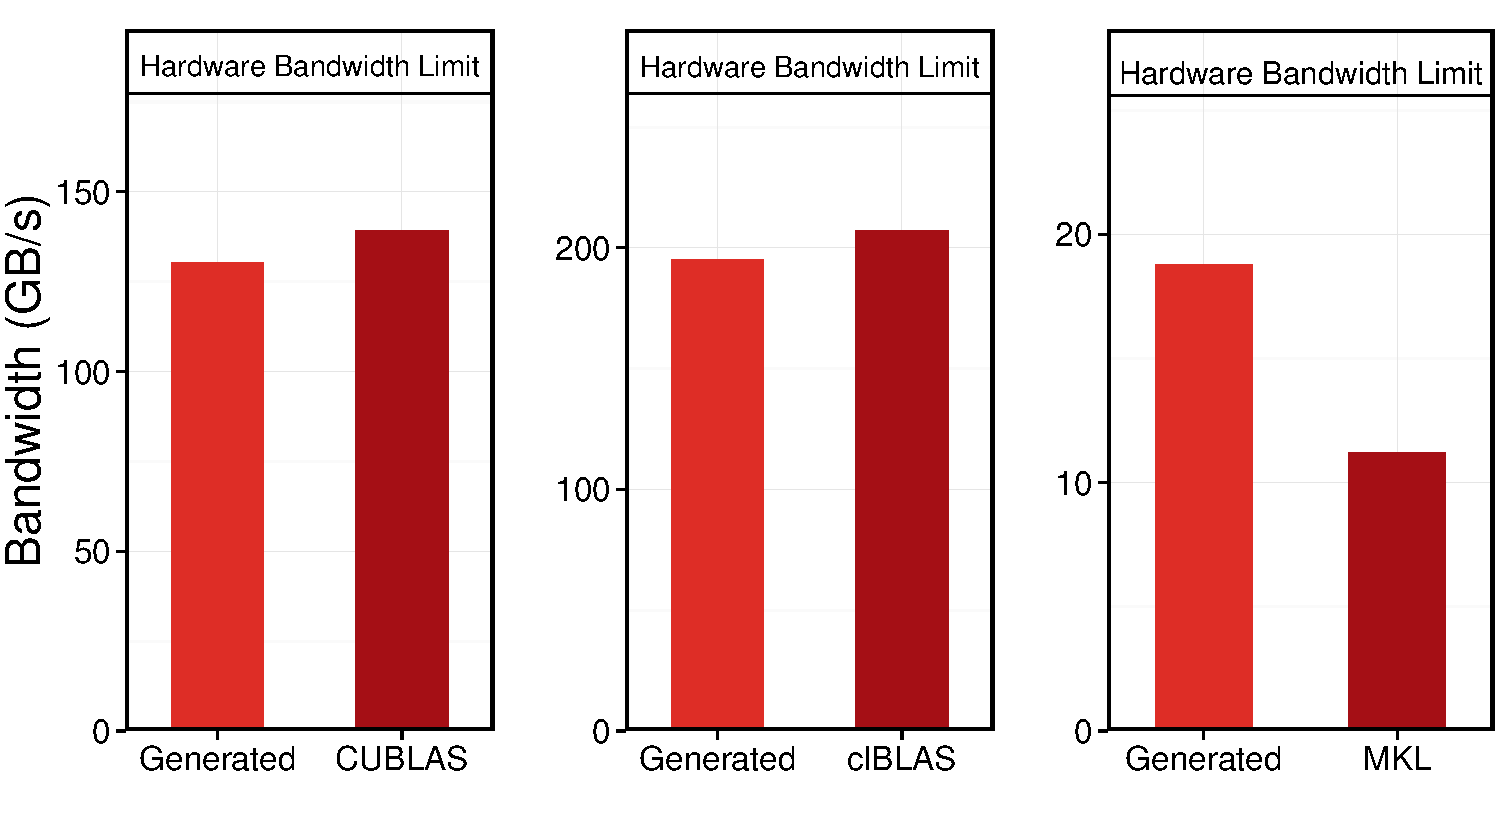
\includegraphics[width=\linewidth]{Plots/ReductionGenerator/reduce_automatic_runtime.pdf}
  \caption{Performance comparisons for code generated for three automatically found low-level expressions against hardware-specific library code on three platforms.}
  \label{fig:reduce:expr:automatic:performance}
\end{figure}

The results shows that the generated code for the automatically found expressions are on par with the \CUBLAS implementation of Nvidia and the \clBLAS implementation of AMD achieving about 95\% of their performance.
On the Intel platform our generated code actually outperforms the \MKL implementation.
This is due to the implementation of \MKL and the particular multi-core \CPU used in the experiments.
For the \emph{asum} benchmark the \MKL implementation does not use thread level parallelism, presumably with the assumption that \emph{asum} is a memory bound benchmark.
The used multi-core \CPU is actually a two socket machine where two chips are combined on a single motherboard.
In this configuration there are two memory controllers available -- one for each socket.
Therefore, thread level parallelism is actual beneficial for the \emph{asum} benchmark on this particular hardware giving our generated code a speedup of 1.67.

The three plots together also show that our approach offers true performance portability.
While each individual \BLAS implementation is not-portable and bound to a specific hardware architecture, our system automatically searched and found three expressions systematically derived from a single high-level representation which offer high performance on all three platforms.
With our approach we achieve the same relative performance on all platforms which is within 75\% of the corresponding hardware bandwidth limit.

\begin{figure*}[p]
%
\centering
\begin{subfigure}[b]{0.65\linewidth}
\includegraphics[width=\linewidth]{nv\string_search.pdf}
\caption{Nvidia \GPU}
\label{fig:search:nv}
\end{subfigure}
\\
%
\begin{subfigure}[b]{0.65\linewidth}
\includegraphics[width=\linewidth]{amd\string_search.pdf}
\caption{AMD \GPU}
\label{fig:search:amd}
\end{subfigure}
\\
%
\begin{subfigure}[b]{0.65\linewidth}
\includegraphics[width=\linewidth]{intel\string_search.pdf}
\caption{Intel \CPU}
\label{fig:search:intel}
\end{subfigure}

\caption[Search efficiency of our prototype search tool]{
   Search efficiency.
   The vertical partitioning represents the number of fixed derivations in the search tree.
   The red line connects the fastest expressions found so far.
}
\label{fig:search}
\end{figure*}


\paragraph{Search Efficiency}
We now investigate the efficiency of our simple search strategy.
\autoref{fig:search} shows how many expressions were evaluated during the search.
The evaluated expressions are grouped from left to right by the number of rules applied in the search tree.
The red line connects the fastest expression found so far.

As can be seen the performance improves steadily for all three platforms before reaching a plateau.
For both \GPUs the best performance is reached after testing about 40 expressions.
At this point we have fixed five derivations and found a subtree offering good performance for some expressions.
Nevertheless, even in the later stages of the search many expressions offer poor performance, which is mainly due to the sensitivity of \GPUs for selecting appropriate numerical parameters.
On the \CPU performance converges after testing about 20 expressions and more expressions offer good performance.
This shows that for this particular benchmark the \CPU is easier to optimize for and not as sensitive when selecting numerical parameters.
Overall the search took less than one hours on each platform.

\bigskip

\noindent
These results show, that applying our rules automatically is feasible and capable of finding high performing low-level expressions for high-level expressions written by the programmer.
Our approach offers true performance portability where the portable high-level expression is systematically and automatically optimized for a particular hardware architecture delivering similar relative performance on all tested devices.
Nevertheless, we only tested our simple automatic search strategy with the parallel reduction as a single benchmark.
For more complex applications the search space becomes bigger and more advanced search techniques have to be applied.
We intend to explore this topic in the future, as we will discuss in more detail in \autoref{section:future-work}.




\section{Linear Algebra Applications}

In this section we evaluate four linear algebra applications: scaling a vector with a constant ($scal$), summing up the absolute values of a vector ($asum$), computing the dot product of two vectors ($dot$), and performing a matrix vector multiplication ($gemv$).
We have performed experiments with two input sizes.
For $scal$, $asum$ and $dot$, the small input size corresponds to a vector size of 64MB.
The large input size uses 512MB (the maximum \OpenCL buffer size for our platforms).
For $gemv$, we use an input matrix of 4096$\times$4096 elements (64MB) and a vector size of 4096 elements (16KB) for the small input size.
For the large input size, the matrix size is 8192$\times$16384 elements (512MB) and the vector size 8192 elements (32KB).

We choose linear algebra kernels as benchmarks, because they are well known, easy to understand, and used as building blocks in many other applications.
\autoref{lst:linear-algebra-expr} shows how the benchmarks are expressed using our high-level patterns.
% we express vector scaling, sum of absolute values, dot product and matrix vector multiplication using our high-level patterns.
While the first three benchmarks perform computations on vectors, matrix vector multiplication illustrates a computation using 2D data structures.

For scaling (\autoref{lst:linear-algebra-expr:scal}), the \map pattern is used for multiply each element with a constant $\alpha$.
%applies a function to each element which multiplies it with a constant $\alpha$.
The sum of absolute values (\autoref{lst:linear-algebra-expr:asum}) and the dot product (\autoref{lst:linear-algebra-expr:dot}) applications both perform a summation, which we express using the \reduce pattern customized with the addition.
For dot product, a pair-wise multiplication is performed before applying the reduction expressed using the \zip and \map patterns.

The \autoref{lst:linear-algebra-expr:gemv} shows matrix vector multiplication as defined in \BLAS: $\vec{y} = \alpha A \vec{x} + \beta \vec{y}$.
To multiply the matrix $mat$ with the vector $xs$, the \map pattern maps the computation of the dot-product with the input vector $xs$ to each row of the matrix $mat$.
Afterwards the resulting vector is added to the scaled vector $ys$ using the \zip and \map patterns.
Notice how we are reusing the expressions for dot-product and scaling as building blocks for the more complex matrix-vector multiplication.
This shows one strength of our system: expressions describing algorithmic concepts can be reused, without committing to a particular low-level implementation.
The dot-product from $gemv$ may be implemented in a totally different way from the stand-alone dot-product.

\begin{lstlisting}[%
  float,%
  caption={Linear algebra kernels from the \BLAS library expressed using our high-level algorithmic patterns.},%
  label={lst:linear-algebra-expr},%
  lineskip={1em}% TODO: smaller skip before last line
  ]
$scal\ \alpha\ xs = \map\ (\lambda\ x.\ \alpha \times x)\ xs\label{lst:linear-algebra-expr:scal}$
$asum\ xs   = \reduce\ (+)\ 0\ (\map\ abs\ xs)\label{lst:linear-algebra-expr:asum}$
$dot\ xs\ ys  = \reduce\ (+)\ 0\ (\map\ (\times)\ (\zip\ xs\ ys))\label{lst:linear-algebra-expr:dot}$
$gemv\ mat\ xs\ ys\ \alpha\ \beta =\label{lst:linear-algebra-expr:gemv}$                    $\map\ (+)\ \big(\zip\ (\map\ (scal\ \alpha \circ dot\ xs)\ mat)\ (scal\ \beta\ ys) \big)$
\end{lstlisting}
%$\begin{aligned}gemv\ &mat\ xs\ ys\ \alpha\ \beta =\\[-.5em]&\map\ (+)\ \big(\zip\ (\map\ (scal\ \alpha \circ dot\ xs)\ mat)\ (scal\ \beta\ ys) \big)\end{aligned}$




\subsection{Comparison vs. Portable Implementation}


First, we show how our approach performs across our three test platforms.
We use the \BLAS \OpenCL implementations written by AMD~\cite{clBLAS} as our baseline for this evaluation since it is implemented in \OpenCL and functionally portable across all test platforms.
\autoref{fig:linear-algebra-expr:clblas} shows the performance of our approach relative to \clBLAS for our four benchmarks.
As can be seen, we achieve better performance than \clBLAS on most platforms and benchmarks.
The speedups are the highest for the \CPU, with up to 20$\times$. % for the $asum$ benchmark with a small input size.
The reason is that \clBLAS was written and tuned specifically for an AMD \GPU which usually exhibit a larger number of parallel processing units as \CPUs.
Our systematically derived expression for this benchmark is tuned for the \CPU avoiding too much parallelism, which is what gives us such large speedup.




\subsection{Comparison vs. Highly-tuned Implementations}

We compare our approach with a state-of-the-art implementation for each platform.
For Nvidia, we pick the highly tuned \CUBLAS implementation of \BLAS written by Nvidia~\cite{cuBLAS}.
For the AMD \GPU, we use the same \clBLAS implementation as before because it has been written and tuned specifically for AMD \GPUs.
Finally, for the \CPU we use the Math Kernel Library (\MKL)~\cite{MKL} implementation of \BLAS written by Intel, which is known for its high performance.

\autoref{fig:linear-algebra-expr:results:nv} shows that the code generated by our approach matches the performance of \CUBLAS for $scal$, $asum$ and $dot$ on the Nvidia \GPU.
For $gemv$ we outperform \CUBLAS on the small size by 20\% while we are within 5\% for the large input size.
Given that \CUBLAS is a proprietary library highly tuned for Nvidia \GPUs, these results show that our technique is able to achieve high performance.

\begin{figure}[t]
  \centering
  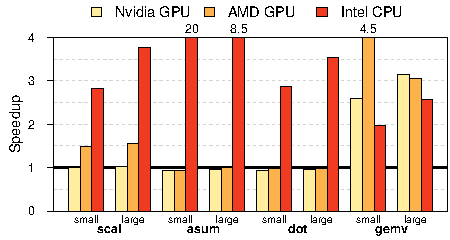
\includegraphics[width=.8\linewidth]{Plots/LA/LA_vs_clBLAS.pdf}
  \caption[Performance of our approach relative to a portable \OpenCL reference implementation]%
          {Performance of our approach relative to a portable \OpenCL reference implementation (\clBLAS).}
  \label{fig:linear-algebra-expr:clblas}
\end{figure}

On the AMD \GPU, we are surprisingly up to 4.5$\times$ faster than the \clBLAS implementation on $gemv$ small input size as shown in \autoref{fig:linear-algebra-expr:results:amd}.
The reason for this is the way how \clBLAS is implemented:
\clBLAS generates the \OpenCL code using fixed templates and in contrast to our approach, only one implementation is generated since they do not explore different pattern compositions.

For the Intel \CPU (\autoref{fig:linear-algebra-expr:results:intel}), our approach beats \MKL for one benchmark and matches the performance of \MKL on most of the other three benchmarks.
For the small input sizes on the $scal$ and $dot$ benchmarks we are within 13\% and 30\% respectively.
For the larger input sizes, we are on par with \MKL for both benchmarks.
The $asum$ implementation in the \MKL does not use thread-level parallelism, while our implementation does and, thereby, achieves a speedup of up to 1.78 on the larger input size.


\begin{figure*}[p]
  \centering
  \begin{subfigure}[b]{0.65\linewidth}
    \includegraphics[width=\linewidth]{PLDI2015/application\string_results\string_vs\string_BEST\string_nv}
    \caption{Nvidia \GPU}
    \label{fig:linear-algebra-expr:results:nv}
  \end{subfigure}
  \\
  \begin{subfigure}[b]{0.65\linewidth}
    \includegraphics[width=\linewidth]{PLDI2015/application\string_results\string_vs\string_BEST\string_amd}
    \caption{AMD \GPU}
    \label{fig:linear-algebra-expr:results:amd}
  \end{subfigure}
  \\
  \begin{subfigure}[b]{0.65\linewidth}
    \includegraphics[width=\linewidth]{PLDI2015/application\string_results\string_vs\string_MKL\string_intel}
    \caption{Intel \CPU}
    \label{fig:linear-algebra-expr:results:intel}
  \end{subfigure}
  \caption[Performance comparison with state-of-the-art, platform-specific libraries]%
          {Performance comparison with state-of-the-art, platform-specific libraries: \CUBLAS for Nvidia, \clBLAS for AMD, \MKL for Intel.
           Our approach matches the performance on all three platforms and outperforms \clBLAS in some cases.
         }
   \label{fig:linear-algebra-expr:results}
\end{figure*}

\section{Molecular Dynamics Physics Application}

The molecular dynamics (\MD) application is a physics simulation taken from the {\small SHOC}~\cite{DanalisMMMRSTV10} benchmark suite.
It calculates the sum of all forces acting on a particle from its neighbors.
\autoref{lst:md} shows the implementation using our high-level patterns.

The function $updateF$ (\autoref{lst:md:updateF}) updates the force $f$ influencing particle $p$ by computing and adding the force between particle $p$ and one of its neighbors.
Using the neighbor's index $nId$ and the vector storing all particles $ps$, the neighboring particle is accessed (\autoref{lst:md:access}) and the distance between the particle $p$ and its neighbor $n$ is computed (\autoref{lst:md:distance}).
If the distance is below threshold $t$, the force between the two particles is calculated and added to the overall force $f$ (\autoref{lst:md:update}).
If the distance is above the threshold, the force is not updated (\autoref{lst:md:noUpdate}).

For computing the force for all particles $ps$, we use the \zip pattern~(\autoref{lst:md:zip}) to build a vector of pairs, where each pair combines a single particle with the indices of all of its neighboring particles ($p$ and $ns$ in \autoref{lst:md:md}).
The function which is applied to each pair by the \map pattern in \autoref{lst:md:md} is expressed as a lambda expression.
Computing the resulting force exerted by all the neighbors on one particle is done by applying the \reduceSeq pattern on the vector $ns$ storing the neighboring indices.
We use function $updateF$ inside the reduction to compute the force for each particle with index $nId$ and add it to the overall force on $p$.
% As $updateF$ is not associative we have to use the sequential version of reduce.

We use lambda expressions for binding of additional information as arguments to functions.
This example shows that our patterns can be used to implement not only simple benchmark applications.


\begin{lstlisting}[%
  float,%
  caption={Molecular dynamics physics application expressed using our high-level algorithmic patterns.},%
  label={lst:md}%
  ]
$updateF\ f\ nId\ p\ ps\ t =\label{lst:md:updateF}$
  $\textit{let}\ n = ps[nId]\label{lst:md:access}$
  $\textit{let}\ d = calculateDistance\ p\ n\label{lst:md:distance}$
  $\textit{if}\ (d < t)\ f + (calculateForce\ d)\label{lst:md:update}$
  $\textit{else}\ f\label{lst:md:noUpdate}$

$md\ ps\ nbhs\ t = \map\ \big(\lambda\ p,ns.\label{lst:md:md}$
    $\reduceSeq\ (\lambda\ f,nId.\ updateF\ f\ nId\ p\ ps\ t)\ 0\ ns$
  $\big)\ (zip\ ps\ nbhs)\label{lst:md:zip}$
\end{lstlisting}

\begin{figure}[t]
  \centering
  \begin{subfigure}[b]{0.48\linewidth}
    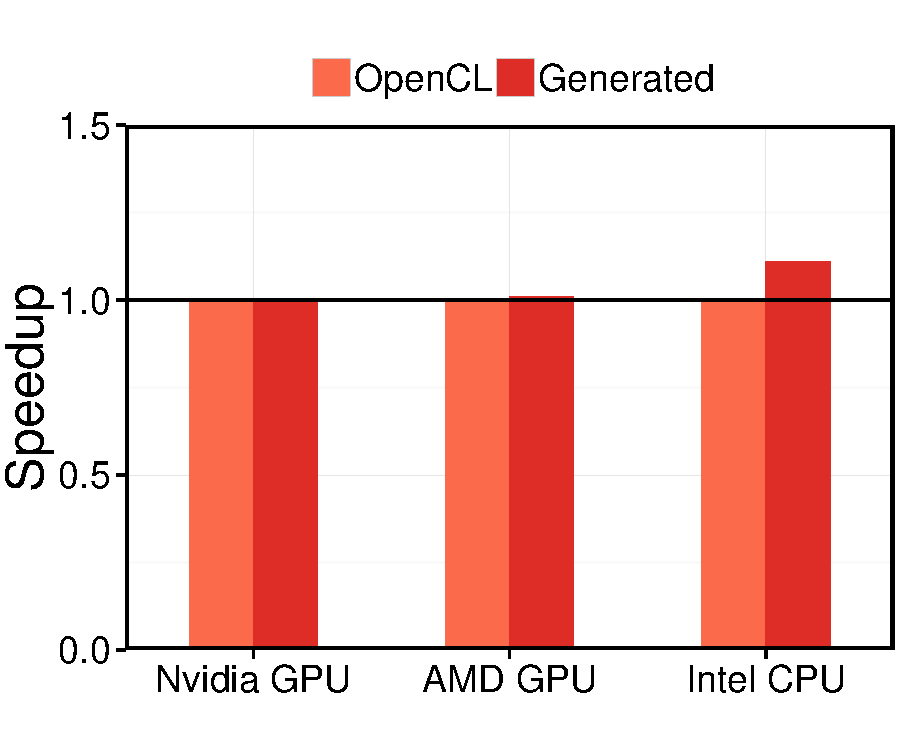
\includegraphics[width=\linewidth]{Plots/MD/md_speedup.pdf}
    \caption{Molecular Dynamics}
    \label{fig:md:results}
  \end{subfigure}
  \hfill
  \begin{subfigure}[b]{0.48\linewidth}
    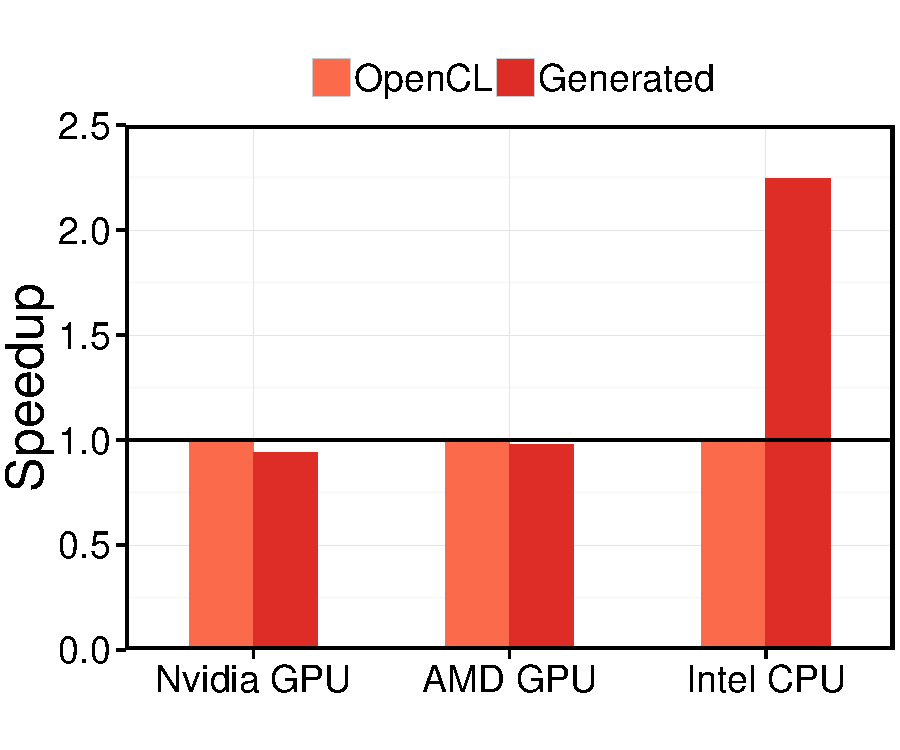
\includegraphics[width=\linewidth]{Plots/BlackScholes/bs_speedup.pdf}
    \caption{BlackScholes}
    \label{fig:blackScholes:results}
  \end{subfigure}
  \caption[Performance of our approach relative to native \OpenCL implementations of the \MD and BlackScholes benchmarks]%
          {Performance of our approach relative to portable \OpenCL implementations of the \MD and BlackScholes benchmarks.}
   \label{fig:bs:ms:results}
\end{figure}

We performed measurements with an input size of 12288 particles for all three test platforms.
The results are shown in \autoref{fig:md:results}.
We can see that the automatically generated \OpenCL code performs very close to the native \OpenCL implementation and is even slightly faster on the Intel \CPU.



\section{Mathematical Finance Application}

\begin{lstlisting}[%
  float,%
  caption={BlackScholes mathematical finance application expressed using our high-level algorithmic patterns.},%
  label={lst:blackScholes}%
  ]
$BSComputation\ s =\label{lst:blackScholes:bscomp}$
  $\textit{let}\ d1 = compD1\ s\label{lst:blackScholes:d1}$
  $\textit{let}\ d2 = compD2\ d1\ s\label{lst:blackScholes:d2}$
  $( compCallOption\ d1\ d2\ s,\ comPutOption\ d1\ d2\ s )\label{lst:blackScholes:return}$

$blackScholes\ stockPrices = \map\ BSComputation\ stockPrices\label{lst:blackScholes:map}$
\end{lstlisting}

The \emph{BlackScholes} application uses a Monte Carlo method for option pricing and computes for each stock price $s$ a pair of call and put options.
\autoref{lst:blackScholes} shows the BlackScholes implementation, where the function defined in \autoref{lst:blackScholes:bscomp} computes the call and put option for a single stock price $s$.
Two intermediate results $d1$ (\autoref{lst:blackScholes:d1}) and $d2$ (\autoref{lst:blackScholes:d2}) are computed and used to compute the two options, which are returned as a single pair (\autoref{lst:blackScholes:return}).
%The computational functions $compD1$, $compD2$, $compCallOption$, and $compPutOption$ are not shown here since they only contain purely sequential code.
In \autoref{lst:blackScholes:map} the $BSComputation$ function is applied to all stock prices (stored in the vector $stockPrices$) using the \map pattern.


\autoref{fig:blackScholes:results} shows the result compared to an \OpenCL implementation of the BlackScholes model provided by Nvidia as part of their software development kit~\cite{NvidiaSDK}.
We measured the runtime on all three test platforms for a problem size of 4 million stock prices.
We see that our approach is on par with the performance of the Nvidia implementation on both \GPUs.
On the \CPU, we actually achieve a 2.2$\times$ speedup due to the fact that the Nvidia implementation is tuned for \GPUs while our implementation generates different code for the \CPU.







\section{Conclusion}

In this chapter we have evaluated the code generation approach introduced in \autoref{chapter:codeGeneration}.
We have seen that our approach successfully addresses the performance portability challenge and generates code which achieves high performance on three distinct hardware platforms: a Nvidia \GPU, an AMD \GPU, and an Intel \CPU.
Furthermore, the comparison against the highly tuned \BLAS libraries shows that our code generator can produce highly efficient code for high-level expressions by systematically transforming them into low-level expressions before compilation.

We have successfully addressed a drawback of \SkelCL which we could not use for implementing an efficient implementation of the \emph{asum} and the dot product benchmarks.
The performance of the code generated by our novel code generation technique is comparable to the best implementations available, as our code generation approach fuses patterns and generates efficient kernels for these two benchmarks.

Finally, we presented a prototype tool which automatically applies the rewrite rules and was able to find implementations with high performance for the parallel reduction on all three tested platforms.
The found expressions were significantly different from the implementations developed by Nvidia, but still achieved high performance exploiting 75\% of the available hardware bandwidth on Nvidia's and AMD's \GPUs as well as on Intel's \CPU.

\bigskip

This concludes the two main technical parts of the thesis.
In the next part we will summaries our work and contributions, discuss how the two presented projects relate to each other and how they can be combined and improved in the future.
Finally, we will conclude the thesis with a comparison against related work.

